\section{\AVOIRmethodname{} Framework}
\label{sec:theoretical}
%\pmcomment{1) Language spec, 2) inference of confidence rules 3) Define confidence sets/bounds, 4) Describe our algorithm, 5) show that our setting is a confidence set, 6) Prove that our method is better 7) Concrete Example}
\subsection{Language Specification}
\label{sec:theoretical:specification}

 
%Following~\cite{albarghouthi2019fairness}, for demonstrating its use, we build our framework as a library for specifying fairness criteria as decorators over python functions. 
We describe \AVOIRmethodname{}'s Domain Specific Language (DSL) used for specifying fairness metrics.
Concrete examples of implemented specifications in \AVOIRmethodname{}'s DSL are provided in Section~\ref{sec:casestudy}.
We focus on binary decision making functions; their outputs can be characterized by Bernoulli r.v.s.
Note that for such a Bernoulli r.v. $X$, $\E[X] = \Pr[X = 1]$ and hereafter, these are used interchangeably. 
Fairness specifications are implemented as decorators over decision functions.
Consider a decision function $f: X \rightarrow \{0, 1\}$, where $X = (X_1, \dots, X_k)$ denotes a real-valued input vector.  We use $R = f(X)$ to simplify the remainder of the definitions. 
\begin{itemize}
    \item  To support expressions beyond those that produce binary outputs, we use the grammar to construct Bernoulli r.vs. For example, a $\nu$-threshold based real-valued output, $R' = (R > \nu)$ and a multi-class output, for class $j$,  $R' = (R == j)$ correspond to Bernoulli r.vs.
\todo{Expanded definitions}
    \item  Expressions involving $R$ and $X_i$ act as the arguments \lstinline{<E>} to construct an \lstinline{<ETerm>}. For example  $\E[R > 0 | X_1 + X_2 > a]$ is an \textit{elementary subexpression} and an \lstinline{<ETerm>}
\end{itemize}
$c$ terms represent constant real values, used, for example, as bounds for expressions.
The grammar provided in Figure~\ref{fig:grammar} can be then used to construct various group fairness criteria.
%Nonparametric confidence sequences~\cite{howard2021time} can be used to extend these results to other r.vs.
%The grammar can be described using a Dmain Specific Language (DSL).
%\paragraph{Grammar for Specification DSL} 
%We start with the grammar used by prior work and enhance the grammar to simplify the expressions used for common fairness specifications. 
%Figure~\ref{fig:grammar} describes the full grammar. 
%\subsubsection{Modified Grammar}
We modified the grammar from prior work to include two additional operations. 
First, we added a \texttt{given} argument to the expectation term, which allows a user to specify conditional probabilities directly, in contrast to specifying it as a ratio of joint/marginal probabilities. 
 %In \citet{albarghouthi2019fairness}, conditional probabilities need to be specified as a ratio of the joint probability divided by the marginal probability of the conditional, i.e., $\E(A|B)$
 \begin{align*}
     \frac{\E(A \vee (B=b))}{\E(B=b)} \rightarrow \E(A, \mathtt{given}=(B=b))
 \end{align*}
 which is used to represent $\E[A|B=b]$, simplifying expressions used for group fairness specification.
Additionally, we add binary comparison operators $<, >, ==, !=$, which further simplifies the process of writing specifications. %\citet{albarghouthi2019fairness} only consider the $>$ operator as a part of their grammar. Thus, we build a more expressive grammar.

\subsection{Propagating Bounds}
\label{sec:theoretical:propagation}
%\paragraph{Inference and Optimization}
Generating the bounds for a specification requires propagating guarantees from elementary subexpressions.
Assuming that observed values for each \texttt{<E>} correspond to an underlying random variable $X$,
a probabilistic guarantee $\phi_X$ consists of an empirical estimate $\BarE[X]$, a concentration bound $\epsilon_X$, and a failure probability $\delta_X$, such that $\Pr[|\E[X] - \BarE[X]|\geq \epsilon_X] \leq \delta_X$.
We refer to expressions of this form as \textit{elementary} subexpressions.
A fairness specification will typically consist of multiple such elementary expressions, denoted as {\it compound} expressions.
For compound expressions, we must infer the implied guarantees that can be provided, with corresponding constraints.
%In addition, guarantees may require certain constraints to be satisfied.
Each inference rule corresponds to a derivation in the DSL grammar.
Inference rules have preconditions and postconditions that follow the general expression
\begin{align*}
 \frac{\bigcup \left\{r | r \in \{\phi, \psi, C \}\right\}}{\bigcup \left\{s | s \in \{ \phi, \psi, C \} \right\} }
\end{align*}
where $\phi$ denotes a claim for a subexpression, $\psi$ for a \verb|<spec>|, $\BarE$ and $\epsilon$ are the mean and concentration terms associated with a subexpression claim,  $C$ denotes a constraint. 
\todo{Updated the language to show the assumptions} 
For example, consider starting with the assumptions $X: (\BarE[X], \epsilon_X, \delta_X)$, $Y: (\BarE[Y], \epsilon_Y, \delta_Y)$.
Then we have
\begin{align*}
    |\E[X] \pm  \E[Y] - (\BarE[X] \pm \BarE[Y])| &= |(\E[X] - \BarE[X]) \pm  (\E[Y] - \BarE[Y])| \\
                                                  & \leq |\E[X] - \BarE[X]| + |\E[Y] - \BarE[Y]|\\
                                                  & \leq \epsilon_X + \epsilon_Y
\end{align*}
i.e., we can derive $X \pm Y: \left(\BarE[X] \pm \BarE[Y], \epsilon_X + \epsilon_Y, \delta_X + \delta_Y\right)$.
Some derivations also lead to rules that require constraints.
For instance, assume $X: (\BarE[X], \epsilon_X, \delta_X), \BarE[X] > c$. 
Then we have $\Pr[X < \BarE[X] - \epsilon_X] > 1 - \delta$
If we add the constraint that $\BarE[X] - \epsilon_X \geq c$, we have $\Pr[X < c] > 1 - \delta$, thus, 
\begin{align*}
    X: (\BarE[X], \epsilon_X, \delta_X) \implies \psi \equiv X > c: (T, \delta_X) \\
    \text{under the constraint } \{ \BarE[X] - \epsilon_X \geq c\}
\end{align*}
The full set of inference rules required for the DSL is provided in the appendix (\Figref{fig:inference}).
The implementation in \AVOIRmethodname{} follows these rules but can be extended to other rule inference templates that support the DSL.
We note that these rules extend the ones implemented by VeriFair (VF)\footnote{Verifair}~\citep{bastani2019probabilistic} with constraints that enable the optimizations required in \AVOIRmethodname{} (see Appendix~\ref{sec:appendix:inference-rules}). 
%\pmcomment{SP: Point to appendix?}

%\pmcomment{Keep constraint rules}




\subsection{Optimizing Bounds}
\label{sec:theoretical:optimization}


\subsubsection{\AVOIRmethodname{} Algorithm}

%\pmcomment{Move to algorithm environment}
%\pmcomment{reference MLP and interior point methods}
The pseudocode for the optimization procedure in \AVOIRmethodname{} is described in  the appendix (Algorithm~\ref{alg:method}).
The input to the algorithm is the reporting threshold probability $\Delta$ and a specification $\psi$.
We then infer a symbolic optimization problem is inferred corresponding to the failure probabilities and constraints derived from concentration bounds.
At each step, the \texttt{OBSERVE(X)} function is called with new observation of every \textit{elementary} subexpression and observed output.
The running mean and counts of observations are updated.
The final optimization problem \texttt{OPT} corresponding to each specification is a nonlinear constrained optimization problem.
We use the COIN-OR implementation of IPOPT~\citep{wachter2006implementation}, accessed though the Pyomo~\citep{hart2011pyomo} interface to solve this problem at each step.
If a solution is successfully found for \texttt{OPT}, the algorithm terminates, with the estimate for the specification having reached the required threshold.
If no solution is found, the estimates continue to be updated with $\delta_i = \Delta$ for each \textit{elementary} subexpression.
The main intuition behind the algorithm is to create a confidence sequence corresponding to the estimates at each time step.
The \texttt{OPT} corresponding to a specification:
\begin{align}
    \label{eq:optimization}
    \begin{split}
        &\min_{\delta_i} \sum_{i=1}^{n}\delta_i  \\
        \text{s.t. } &g_k(\delta_{1, \dots, n}, \BarE[X_1], \dots, \BarE[X_n]) \leq \epsilon_k\\
        & 0 \leq \delta_i \leq 1
    \end{split}
\end{align}
where $g_k$ and $\epsilon_k$ are the functions/bounds derived using the transformations carried out through the DSL inference rules (further details in Appendix~\ref{sec:appendix:inferrence-rules:opt}).


\begin{definition}
For $\delta \in (0, 1)$, a $(1-\delta)$ \textit{confidence sequence} is a sequence of confidence sets, usually intervals  $(\rm{CI}_t)_{t=1}^\infty,$, say $\rm{CI}_t \eqdef (L_t, R_t) \subseteq \sR$ satisfying a uniform convergence guarantee. After observing the $t$th unit, we calculate an updated confidence set $\rm{CI}_t$ for an unknown quantity of interest $\theta_t$ with the coverage property $\Pr(\forall t \geq 1, \theta_t: \theta_t \in \rm{CI}_t) \geq 1 - \delta$~\citep{howard2021time}.
\end{definition}

In this paper, we focus on the mean of r.v.s $\E[X]$ that constitute estimates for \textit{elementary} subexpressions as the quantities of interest. 
We use adaptive concentration inequalities to construct these confidence sequences.
Any adaptive concentration inequality that can be applied to a r.v. $X \in \{0, 1\}$ such that 
\begin{equation}
    \Pr[|\BarE_t[X] - \E[X]| \geq \epsilon(t, \delta)] \leq \delta
    \label{eq:adaptive-conc:general}
\end{equation}
can be used in \AVOIRmethodname{}. 
Here, $\BarE_t[X]$ denotes the empirical estimate of $\E[X]$ after the $t^{\rm{th}}$ observation.
For the purpose of comparison with previous work (eg., VF), we use the Adaptive Hoeffding Inequality~\citep{zhao2016adaptive}, which will be referred to as $\rm{AIN}$ hereafter.
%\pmcomment{SP: refer to $\rm{AIN}$ above but $\rm{AIN}$ below. Check and unify.}

\begin{theorem}
The sequence of estimates generated by \AVOIRmethodname{} form a confidence set.
\label{thm:conf-seq}
\end{theorem}
The proof follows from the fact that \AVOIRmethodname{} always estimates using a failure probability higher than that which is provided by $\rm{AIN}$, and hence applying a union bound ensures that the estimates are a confidence set. 
The full proof is provided in Appendix~\ref{sec:appendix:confseq}.

\begin{corollary}
The estimates for the overall specification $\psi$ form a confidence sequence converging to $\psi: (b, \Delta), b \in \{T, F\}$.
\end{corollary}
\begin{proof}
We initialize the main specification with the required failure probability $\Delta$. 
The termination condition requires $\sum \delta_i \leq \Delta$.
From Theorem~\ref{thm:conf-seq} we can infer that the confidence sequence corresponding to the termination achieves the required threshold $\Delta$, and therefore, is valid.
\end{proof}


\subsubsection{Improvements over Baseline}
In all prior work~\citep{albarghouthi2017fairsquare,albarghouthi2019fairness,bastani2019probabilistic}, $\delta_i$ for each \textit{elementary} subexpressions is set to $\Delta/n$, where $n$ is the number such term in the specification.
\todo{Introduce $A_\delta$ }
This simplification is carried out using the assumption $A_\delta \eqdef \delta_i = \delta_j \forall i, j$ for all \textit{elementary} subexpressions.
As we do not make this assumption, we can prove the following key theorem.

\begin{definition}
We define the specification stopping time $\gT$ for a confidence sequence as the smallest time $t$ such that, given a threshold $\Delta$ and a specification $\psi$, we can terminate any inference algorithm to claim that  $\Pr[\forall t \geq 1, \psi_t = \widehat{\psi}_\gT] \geq 1 - \Delta$, where $\widehat{\psi}_{\gT}$ is the estimate of $\psi$ at time $\gT$.
\end{definition}

\begin{theorem}
\label{theorem:better-stopping}
Given a threshold probability $\Delta$ for a specification $\psi$, let the stopping time for \AVOIRmethodname{} be $\gT$ and stopping time with the $A_\delta$ assumption be $\gT^+$. Then $\gT \leq \gT^+$
\end{theorem}
See Appendix~\ref{sec:appendix:optimality} for the proof.

%\pmcomment{Need to make this argument rigorous}


%\pmcomment{Write this proof replacing AH/Verifair with arbitrary $\rm{IN}$}

\paragraph{Concrete Example}
%\label{sec:theoretical:improvements:concrete}
%\pmcomment{Prior work makes assumptions of equality of unceertainty thresholds; as we do not make this assumption, which allows us to optimize over prior owrk.}
Consider a Bernoulli r.v $R$ corresponding to the output of a binary decision function, with $s$ being an indicator of class membership. 
Let $X = r \vee s$ and $Y = r \vee \neg s$ be r.vs corresponding to a positive decision for the majority and minority classes, respectively. 
Suppose we aim to estimate $\psi \eqdef X - Y < \epsilon_T$

\begin{figure}[ht]
\begin{subfigure}[b]{0.45\linewidth}
\resizebox{\linewidth}{!}{
    \begin{tikzpicture}
        \centering
        \begin{axis}[
                %xtick = \empty,    ytick = \empty,
                grid=both,
                xlabel = {$\delta_X$},
                %x label style = {at={(1,0)},anchor=west},
                ylabel = {$\delta_Y$},
                %y label style = {at={(0,1)},rotate=-90,anchor=south},
                y label style = {rotate=-90},
                axis lines=left,
                xmin=0.03, xmax=0.06,
                ymin=0.04, ymax=0.07,
                label style={font=\Large}
            ]
            \addplot[color=cb-rose,thick,smooth,domain=0:0.1]{x};
            \addlegendentry{$\delta_X = \delta_Y$}
            
            
            \addplot[name path=delta, color=cb-lilac,thick,smooth,domain=0:0.1,forget plot]{0.1-x};
            \path[name path=axis2] (0,0) -- (0.1,0);
            \addplot [
                thick,
                color=cb-lilac,
                fill=cb-lilac, 
                fill opacity=0.05,
                draw=cb-lilac
            ]
            fill between[
                of=axis2 and delta, soft clip={domain=0:0.1}
            ];
            \addlegendentry{$\delta_X + \delta_Y \leq 0.1$};
            
            
            \addplot[name path=constraint,color=cb-brown,smooth,thick,-,domain=0:0.1,forget plot] {24/exp((9/5)*(((0.2 - sqrt(2.6146 + 5*ln(24/x)/9)/(5*sqrt(62)))^2) * 310 - 2.46838))};
            \path[name path=axis3] (0,0.1) -- (1,0.1);
            \addplot [
                thick,
                color=cb-brown,
                fill=cb-brown, 
                fill opacity=0.05,
                draw=cb-brown
            ]
            fill between[
                of=constraint and axis3,
                soft clip={domain=0:0.1}
            ];
            \addlegendentry{$\epsilon_X + \epsilon_Y \leq 0.2$}
        \end{axis}
    \end{tikzpicture}}
        \caption{No solution exists with additional constraint $A_\delta: \delta_X = \delta_Y = \Delta/2$ - common assumption in prior work.}
        \label{fig:theoretical-example}
    \end{subfigure}
    \hfill
    \begin{subfigure}[b]{0.45\linewidth}
        \centering
        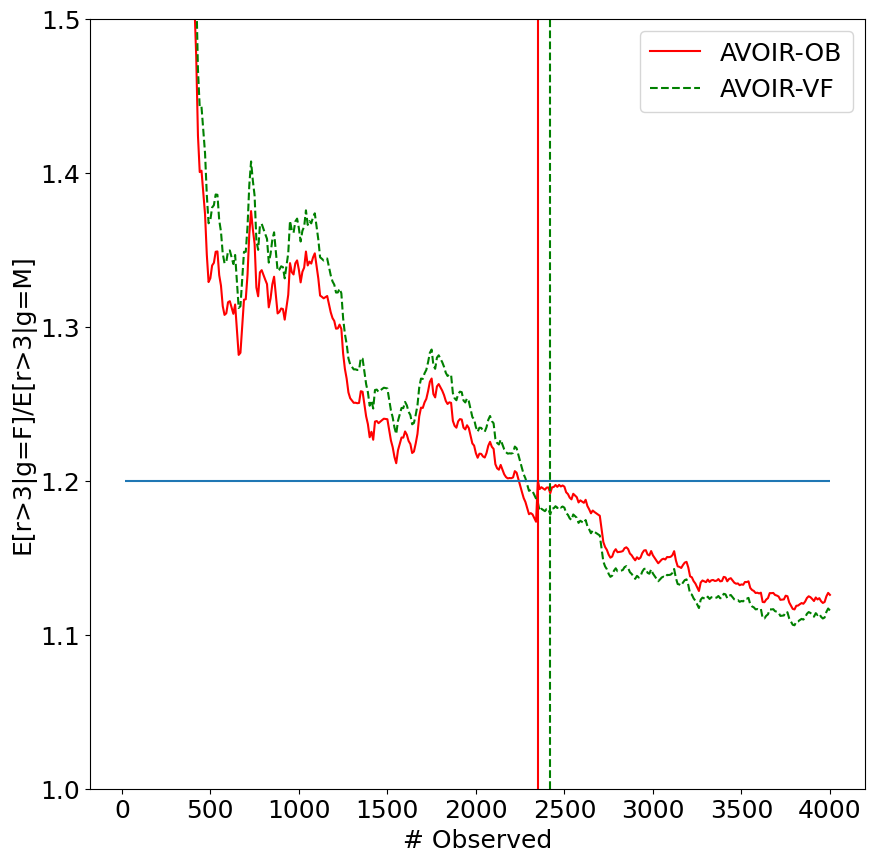
\includegraphics[width=\linewidth]{avoir/images/ratemyprofs.png}
        \caption{Bounds for first half of a gender-fairness specification generated by \AVOIRmethodname{}-OB and AVOIR-VF.}
        \label{fig:casestudy:rmp}
    \end{subfigure}
    \caption{\figleft{} \AVOIRmethodname{} finds a solution for a \textit{theoretical} scenario with $\delta_X + \delta_Y \leq \Delta$ under constraint $\epsilon_X + \epsilon_Y \leq \epsilon_T$ \figright{} For \textit{RateMyProfs}, a real-world dataset, the vertical lines show the step at which the methods can provide a guarantee of failure for the upper bounds with $\Delta <= 0.05$.}
    \label{fig:real-and-theoretical-examples}
\end{figure}


We demonstrate the improvements possible using our approach by instantiating this example with data. 
Suppose we want the upper bound of the failure probability $\Delta = 0.1$ for the specification.
Consider a set of observations such that $\BarE[X] = 0.8, n_X = 1550$ and $\BarE[Y] = 0.5, n_Y = 310$.
Figure~\ref{fig:theoretical-example} shows that no solution is feasible for the optimization problem with $A_\delta$.
However, \AVOIRmethodname{} can find a solution.
For the optimal solution, $\delta_2 \approx 2.35\delta_1$, which aligns with our intuition from section~\ref{sec:related} about allocating higher failure probability to terms with the majority of observations. 
The optimization problem inferred by \AVOIRmethodname{}:
\begin{align}
    \begin{split}
        &\min\limits_{\delta_X, \delta_Y}{\delta_X + \delta_Y} \\
        \text{s.t.  } &\epsilon_X + \epsilon_Y \leq \BarE[X] - \BarE[Y] - \epsilon_T \\
        &0\leq \delta_{X,Y} \leq 1
    \end{split}
\end{align}

%\pmcomment{Please point reader to location in appendix on proof.}


 

\begin{comment}
$\Pr[X] - \Pr[Y]  < \epsilon_T$. 
As $\Pr[X] = \E[X]$ for a Bernoulli r.v., this can be simplified as:
\begin{align*}
    \Pr[\Pr[X] - \Pr[Y] < \epsilon_T] &= \Pr[\E[X] - \E[Y] < \epsilon_T] \\
                                  &= 1 - \Pr[\E[X] - \E[Y] \geq \epsilon_T] \\
\end{align*}

Suppose $\BarE[X]_{(\epsilon_X, \delta_X)}$ and $\BarE[Y]_{(\epsilon_Y, \delta_Y)}$ be statistical guarantees derived for $X$ and $Y$ respectively. 
From the inference rules in Figure~\ref{fig:inference}, we have 
\begin{align*}
    \Pr[|(\E[X]-\E[Y]) - (\BarE[X] - \BarE[Y])| \geq \epsilon_X + \epsilon_Y] &\leq \delta_X + \delta_Y\\
    \implies \Pr[(\E[X]-\E[Y]) \geq \BarE[X] - \BarE[Y] -  (\epsilon_X + \epsilon_Y)] &\leq \delta_X + \delta_Y \\
    \implies \Pr[(\E[X]-\E[Y]) \geq \epsilon_T] &\leq \delta_X + \delta_Y
\end{align*}
where the last inequality follows if $\BarE[X] - \BarE[Y] - (\epsilon_X + \epsilon_Y) \geq \epsilon_T$
\end{comment}


%\pmcomment{TODO: replace the screenshot with a vector graphic from tikz}

\subsection{Visualization for Interactive Refinement}
Using our specification framework as a backend, we built an interactive application for analysis and refinement of specifications provided in our grammar.
Specifically, fairness specifications can be naturally parsed into a tree because of the structure of the grammar.
Each node of the tree represents some sub-expression in the syntax tree of the overall specification.
These nodes allow a user of \AVOIRmethodname{} to interactively audit and tune the specification definition.
To create the visualization, we use Vega~\citep{satyanarayan2015reactive}, a declarative JSON-based visualization grammar.
%To provide the evaluation plots, we need the evaluation values and the observations that they occurred at.
We log the estimates during runs of \AVOIRmethodname{} and then output the grammar in a tabular JSON-format that contains a row for each grammar element and its associated evaluations.
This tabular data is used by our Vega specification to produce the visualizations.
By selecting one of the nodes in the syntax tree, a user can see a plot of the evaluation values associated with the selected grammar element.
This allows for comparison of multiple grammar elements.
The ability to analyze and compare these evaluation values provides context surrounding specification violations, and assists the user in interacting with and deciding how to refine a specification
We provide a detailed example of how these interactions can help \AVOIRmethodname{} users choose an appropriate fairness metric in Section~\ref{sec:casestudy}.
%Given a user provided machine learning model, dataset, and specification the application simulates a stream of observations to the provided model.
%Following the simulation, a visualization is provided that represents the specification as a syntax tree where each node of the tree corresponds to an element of our grammar.
%Figures \ref{fig:casestudy:boston} and \ref{fig:casestudy:adult} show the visualization.
%Note that for each observation made by our machine learning model, the specification is evaluated to check for violations.
%Each grammar element that makes up the specification is evaluated as well, and thus each grammar element is associated with the value it evaluates to for a given observation.
%For the top level specification, \texttt{<spec>}, there is a boolean value associated with each observation, whereas an expectation term, \texttt{<ETerm>}, is associated with a real value.
%We call these plots evaluation plots and two can be observed at a time (see the plots on the right of figure \ref{fig:casestudy:boston}), each with shared scales along the horizontal axis which denotes observations over time.
%The case studies in section \ref{sec:casestudy} demonstrate the usefulness of the context provided by these visualizations.
%To create the visualization, we use Vega \cite{vega}, a declarative JSON-based visualization grammar.
%To provide the evaluation plots, we need the evaluation values and the observations that they occurred at.
%We log these values during the simulation our application runs, and then output the grammar in a tabular JSON-format that contains a row for each grammar element and it's associated evaluations.
%This tabular data is used by our Vega specification to produce the visualizations.
\begin{comment}
The app proceeds in multiple stages,
\begin{enumerate}
    \item First, a user selects a dataset of interest. We built support for two datasets, but our framework is generic enough for any arbitrary csv dataset.
    \item Following this choice, the input variables and output variable for a machine learning model must be specified.
    \item A machine learing model is then selected from a dropdown. We provide support for three models. However, this is for demonstration purposes only - the specification is agnostic to the choice of a machine learning model.
    \item Finally , a specification is input by the user of the app. On the press of a button, the model is trained and then evaluated on the selected dataset. The output monitored by the spec is passed off to the Vega module for further analysis.
\end{enumerate}
\end{comment}